% !TEX encoding = UTF-8
% !TEX TS-program = pdflatex
% !TEX root = ../tesi.tex
%**************************************************************
\chapter{Archittetura del sistema AWMS}
\label{cap:archittettura del sistema AWMS}
%**************************************************************

\intro{In questo capitolo verranno descritti tutte le componenti dell'architettura AWMS e le varie operazioni di comunicazione tra le varie componenti}\\


\section{Descrizione}
Come detto precedentemente dietro alla applicazione mobile c'è tutta un architettura di sistema che permette la comunicazione tra la piattaforma AWMS e l'applicazione mobile con Azzurra.
 
 \begin{figure}[h]
 	\begin{center}
 		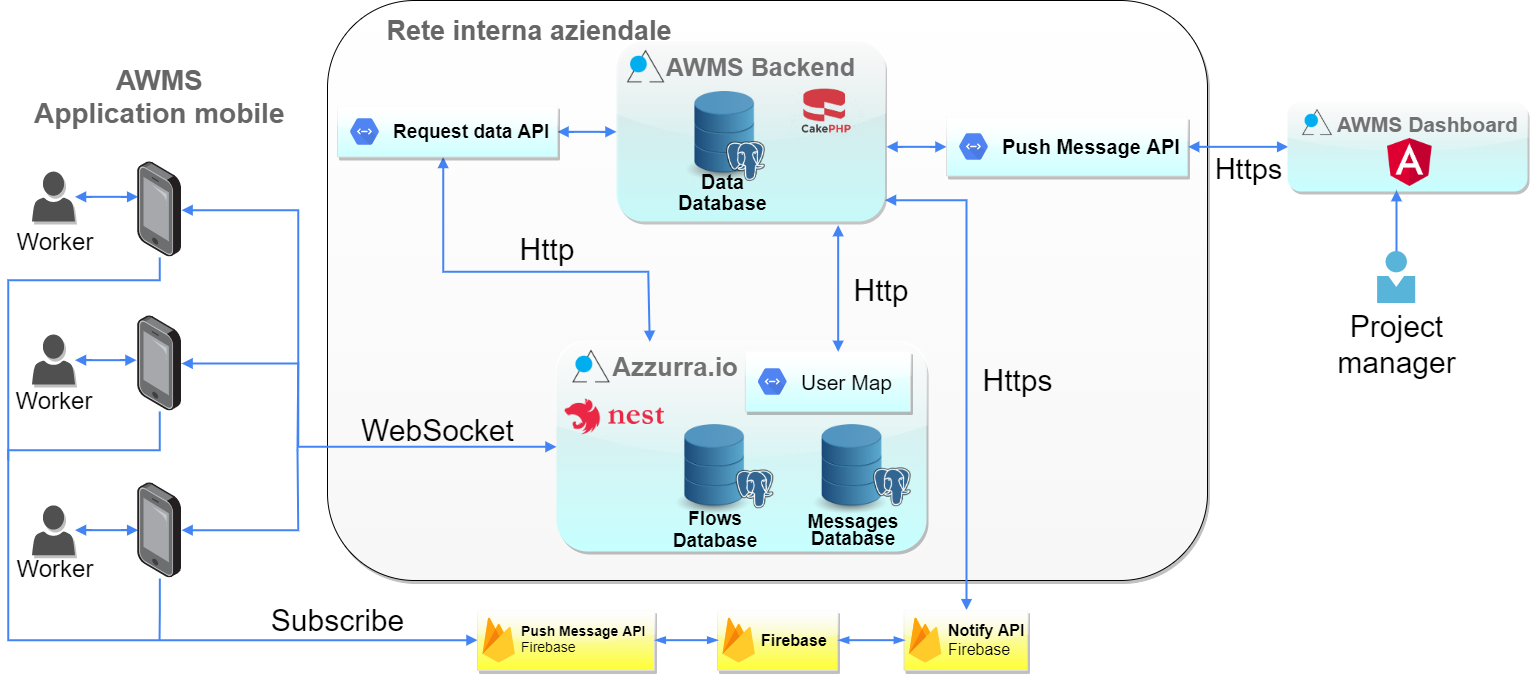
\includegraphics[scale=0.3]{AWMSDiagram.png}
 		\caption{Archittetura di sistema AWMS}
 		\label{fig:arch}
 	\end{center}
 \end{figure}

La figura precedente illustra come è composta l'architettura, e sono cosi descritte:
\begin{itemize}
	\item \textbf{AWMS Dashboard}:È il pannello di controllo attraverso il quale un project manager può interagire con la piattaforma AWMS per poter pianificare il lavoro da svolgere, cioè assegnare un compito alla persona più idonea. Il pannello di controllo è una applicazione web che è stata sviluppata in Angular. La dashboard per comunicare con il back-end, utilizza delle \gls{api}\ap{g} che il back-end espone, quindi per una ragione di sicurezza, back-end e l'applicazione web cioè il front-end, comunicano attraverso \gls{api}\ap{2} con in più l'utilizzo del protocollo di comunicazione HTTPS che cripta la comunicazione. Nella Figura ~\ref{fig:arch} viene mostrato il caso in cui il front-end utilizza \gls{api}\ap{3} per l'invio di notifiche push, questo perché è previsto che una volta il team leader sceglie il lavoratore più idoneo per un certo lavoro, il lavoratore deve essere avvisato, cosi sarà compito del front-end avvisare il back-end che c'è stata una nuova assegnazione e che questa assegnazione deve essere comunicata al diretto interessato attraverso un notifica sull'applicazione mobile con all'interno Azzurra.
\end{itemize}